\begin{frame}
\frametitle{Aufgabe 1a}
\framesubtitle{}
        \begin{itemize}
            \item Durch Abtasten der angelegten Spannung wird der Innenwiderstand des
            DMMs berechnet. 
        \end{itemize}
\end{frame}
\begin{frame}
    \frametitle{Aufgabe 1a}
    \framesubtitle{Schaltplan}
    \begin{figure}[H]
    \begin{center}
        \fbox{
            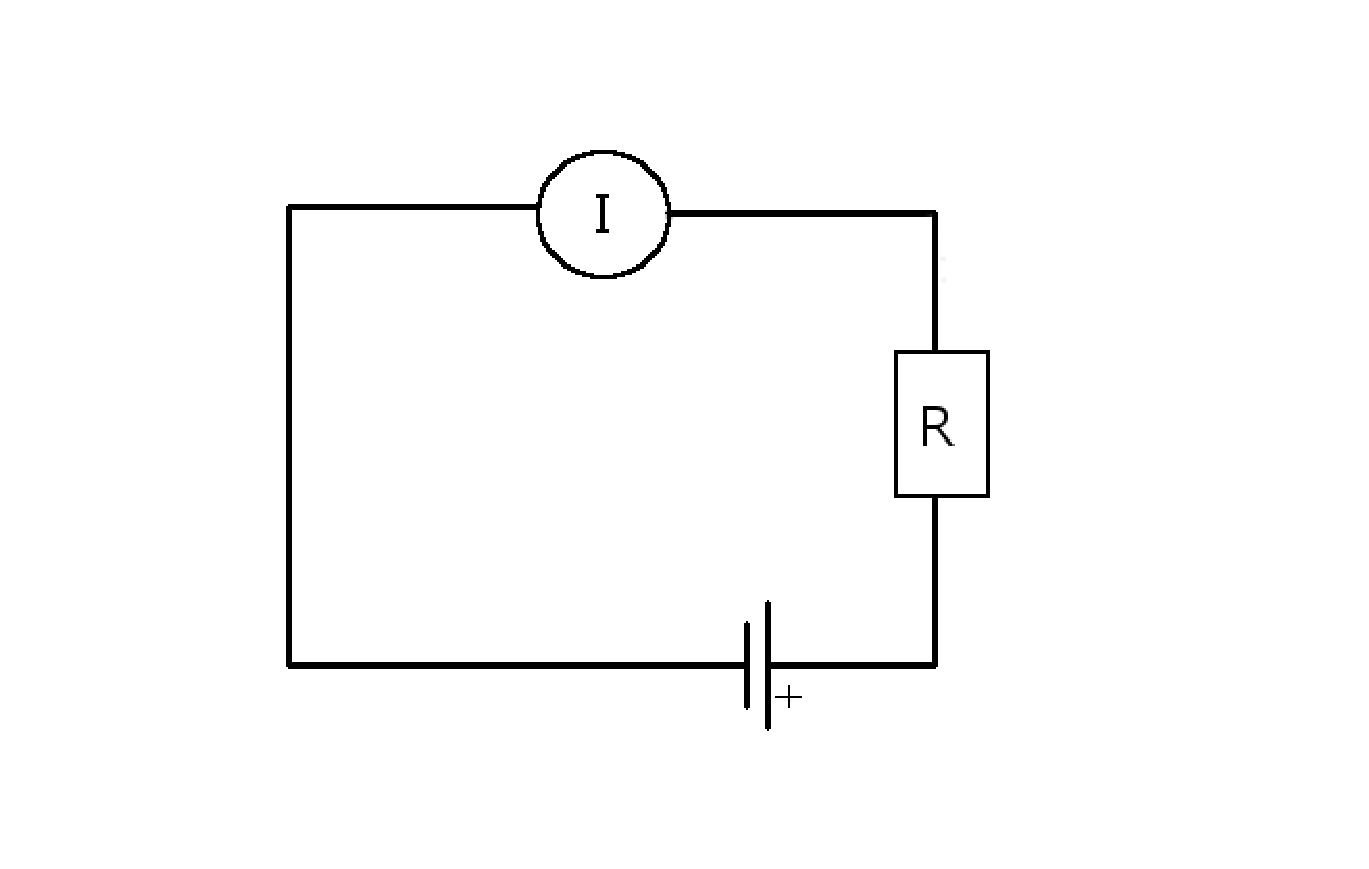
\includegraphics[scale=0.40]{./img/ersatzschaltung.eps}
        }
        \caption{Ersatzschaltung des Messaufbaus}
    \end{center}
    \end{figure}
    
\end{frame}
\begin{frame}
    \frametitle{Aufgabe 1a}
    \framesubtitle{I/U Kennlinie}
    \begin{figure}[H]
    \begin{center}
        \fbox{
            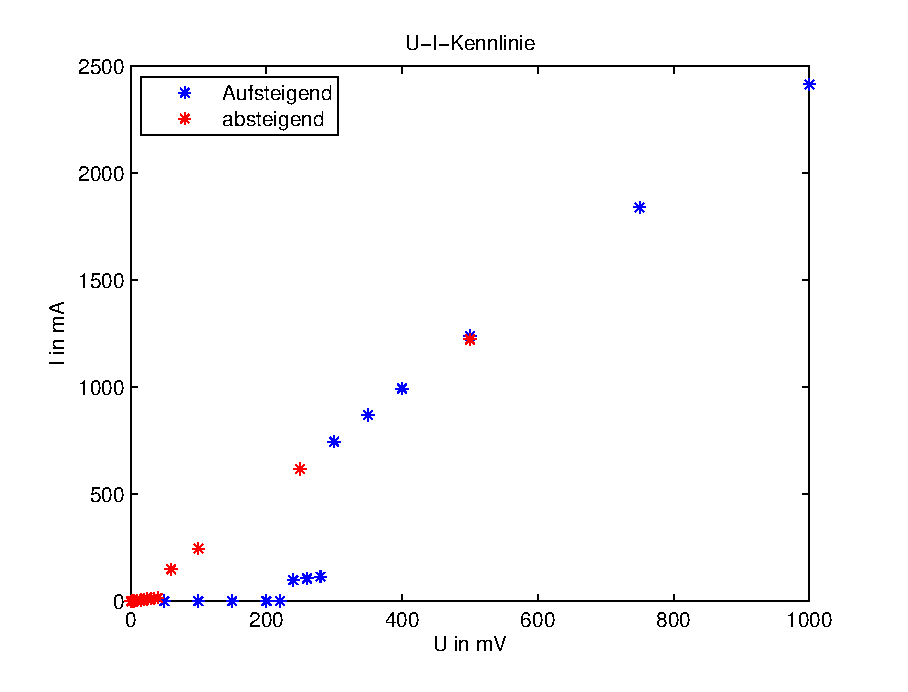
\includegraphics[scale=0.60]{./img/Aufgabe_1a_norm.eps}
        }
    \end{center}
    \end{figure}
\end{frame}
\begin{frame}
    \frametitle{Aufgabe 1a}
    \framesubtitle{I/U Kennlinie}
    \begin{figure}[H]
    \begin{center}
        \fbox{
            \includegraphics[scale=0.65]{./img/Aufgabe_1a_norm_0_20.eps}
        }
    \end{center}
    \end{figure}
\end{frame}
\begin{frame}
    \frametitle{Aufgabe 1a}
    \framesubtitle{Beobachtungen}
    \begin{itemize}
        \item Durch Abtasten der angelegten Spannung wird der Innenwiderstand des
        DMMs berechnet. 
        \item Das Gerät variiert selbständig den Innenwiderstand ('Klicken' beim
        Verändern der Spannung)
    \end{itemize}
\end{frame}
\begin{frame}
\frametitle{Aufgabe 1a}
\framesubtitle{Widerstandssprünge Aufwärts}
    Widerstandsschaltung Aufwärtsmessung:
    \begin{tabular}{c||c|c}
        &Stromstärke Bereich $I/mA$ & Innenwiderstand $R/\Omega$ \\
        \hline
        Hersteller& $0.10 - 1.00$& $200$ \\
        Messwerte & $0.25-1.11$&$199$ \\
        \hline
        Hersteller& $10 -  100$&$2.00$\\
        Messwerte & $98.6-115$&$2.43$ \\
        \hline
        Hersteller& $1000 - 3000$&$0.10$\\
        Messwerte & $746-2415$&$0.40$
    \end{tabular}
\end{frame}
\begin{frame}
\frametitle{Aufgabe 1a}
\framesubtitle{Widerstandssprünge Abwärts}
    Widerstandsschaltung Abwärtsmessung:
    \begin{tabular}{c||c|c}
        &Stromstärke Bereich $I/mA$ & Innenwiderstand $R/\Omega$ \\
        \hline
        Hersteller& $3000-1000$&$0.10$\\ 
        Messwerte & $1224-149$&$0.40$\\
        \hline
        Hersteller& $100-10$&$2.00$\\
        Messwerte & $16.3-1.50$&$2.50$\\
        \hline
        Hersteller& $1.00-0.100$&$200$\\
        Messwerte & $0.01-0.00$&$234.3$
    \end{tabular}
\end{frame}
\begin{frame}
\frametitle{Aufgabe 1a}
\framesubtitle{Interpretation}
    Das Gerät schaltet selbständig Widerstände ein, um
    \begin{itemize}
        \item die Messgenauigkeit bei verschiedenen Widerständen gleich zu
        halten
        \item die Bauteile zu schützen
    \end{itemize}
\end{frame}
